%----------------------------------------------------------------------------------------
%	Chapter 1
%----------------------------------------------------------------------------------------

% To have just one problem per page, simply put a \clearpage after each problem

\section{Aim}
The objective of this project is to predictive the latitude and longitude for a set of test users, given their social friends network and other metadata information as detailed below:

\begin{itemize}
\item A graph of social network, as a tab-delimited file with each line having two user IDs.
\item A training dataset is a csv file of userIds, top 3 hours in GMT where the user make the maximum number of posts during the day and the total number of posts. The training data also contains the lat and lon.
\item The test dataset contains all the fields available in the train dataset except for the latitude and the longitude.
\end{itemize}



\section{Features}
The features available in the data are top 3 hours of the day during which the user posts the maximum number of posts, the total posts per day and  a network of the user's friends. In order to estimate the latitude and the longitude, the set of features of features that best predict these output variables must be identified.  Using features that do not correlate with the output can result in poor prediction.  In order to  identify a possible subset of features that are the best predictors, we could use an intuitive approach of applying  domain knowledge or a more formal approach such as computing correlation or mutual information \cite{Guyon2003}.




\subsection{Feature Selection}
In this project, we have used domain knowledge and visualisation techniques to identify the best predictors.  Intuitively, in most cases, the location of our friends are good indicators of where we are. The next possible indicator is using the hours, given it all in GMT, to calculate longitude as show in \ref{fig:featureHour}. 


\begin{center}
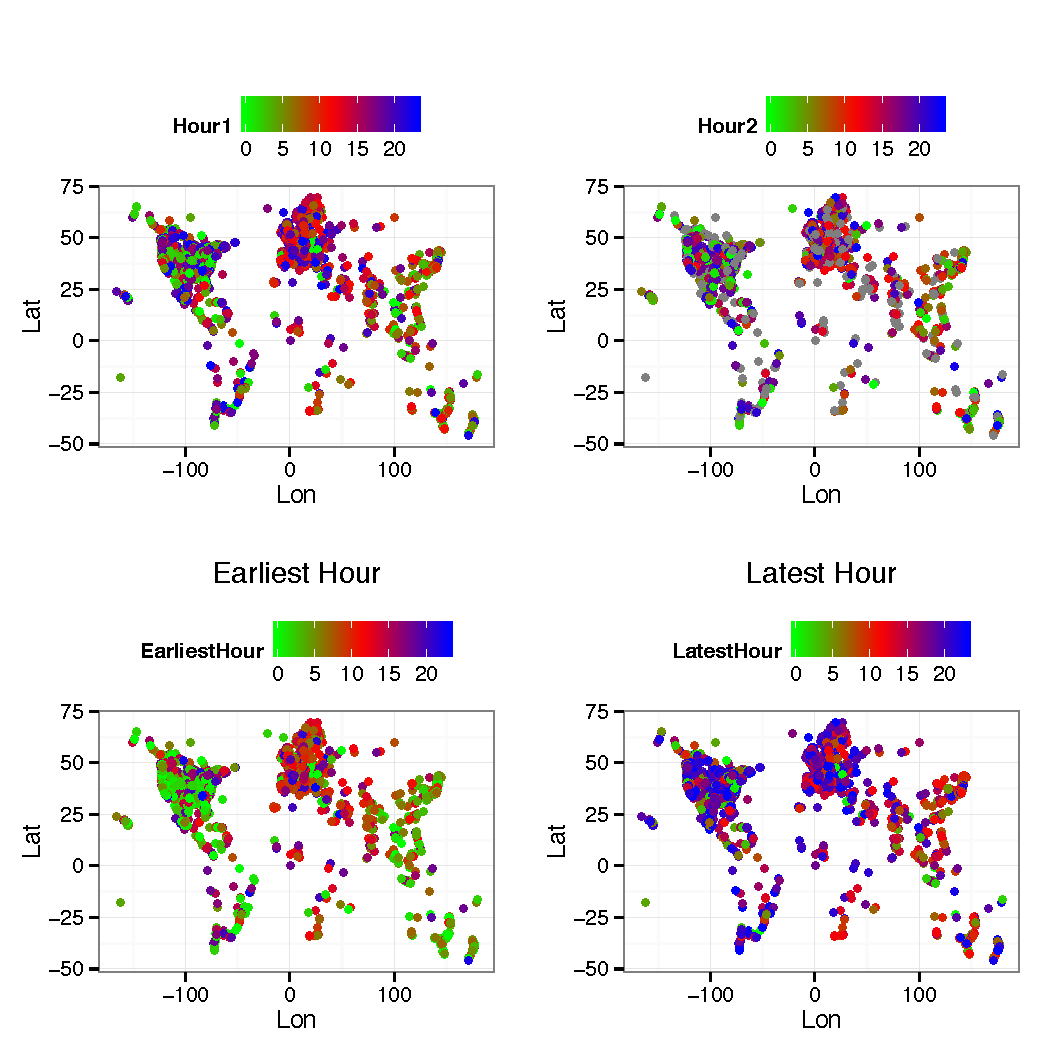
\includegraphics[width=0.75\columnwidth]{figures/featurePlot.pdf} % Example image
\label{fig:featureHour}
\end{center}

\subsection{Feature Transformation}
Although the hours directly do not seem to indicate the longitude, transformating hour1, hour2 and hour2 into earliest and latest hours (min(hour1, hour, hour) \& max (hour,hour2,hour3) are able broadly identify 3 zones , the Americas, Europe \& Africa and AsiaPacific

